\chapter{Elementi Costitutivi}\label{cap:1}

\begin{minipage}{12cm}\textit{
		In questo capitolo si vogliono descrivere e caratterizzare i 3 elementi salienti dell'esperimento:
		\begin{enumerate}
			\item \nameref{Trasformatore}
			\item \nameref{CurrentSense}
			\item \nameref{CurrentDriver}
		\end{enumerate}
	}
Verranno analizzate le loro caratteristiche chiavi per mettere in luce il perché della scelta, e si evidenzieranno eventuali problemi che affliggono in componenti, problemi di cui si è tenuto conto nello sviluppo del progetto per poterli annullare. 
\end{minipage}

%\vspace*{1cm}
\newpage

\section{Trasformatore - Modello di Tokamak}\label{Trasformatore}

Come visto nell'introduzione, la tesi ha come obiettivo la prototipazione del sistema di controllo per le bobine poloidali presenti in impianti tokamak.\\

\begin{figure}[h]
	\centering
	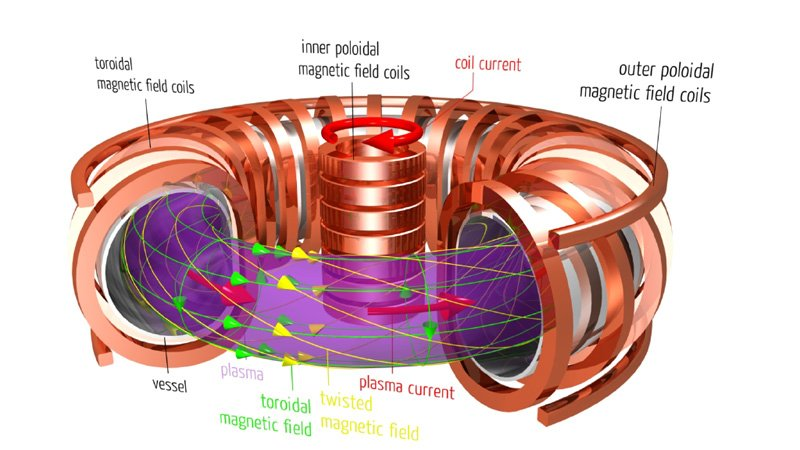
\includegraphics[width=1\textwidth]{Trasformatore/tokamak_scheme.jpg}
	\caption[Schema interno di un Tokamak]{Interno Tokamak}
\end{figure}

\noindent
Le bobine poloidali servono a controllare il plasma presente nel \textit{Vessel} dell'impianto e confinare il Plasma all'interno della camera, cercando al contempo di comprimere il Plasma per realizzare eventi di \textbf{Fusione Nucleare}.\\
L'interazione tra le \textbf{Bobine e Plasma}, ha un modello matematico non dissimile da quello di \textbf{Trasformatore Elettrico} nella relazione Primario-Secondario (con i dovuti paragoni e le ovvie \nonLinearita presenti nel caso di un impianto reale).\\
Grazie a questa similitudine è stato possibile replicare in sicurezza la fisica presente all'interno di un Tokamak, nell'ambiente controllato del laboratorio.\\

\subsection{Modellazione Fisica}

Come descritto nell'articolo di \cite{TokamakCircuit}, è possibile modellare la dinamica tra il Plasma e la Bobina come un circuito la relazione tra un Primario e un Secondario di un Trasformatore.
\begin{figure}[h]
	\centering
	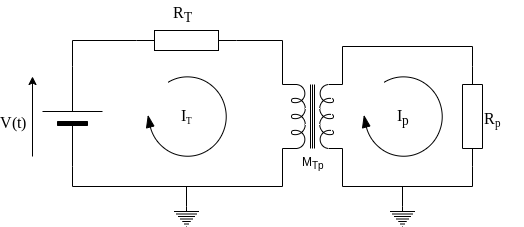
\includegraphics[width=1\textwidth]{Trasformatore/PlasmaCircuit-PlasmaCircuit.png}
	\caption[Circuito Equivalente Bobina/Plasma all'interno di un Tokamak]{Circuito Equivalente Bobina/Plasma}
\end{figure}

\noindent
Sperimentalmente si è in oltre visto che è possibile modellare questa relazione tra i 2 circuiti trascurando le forze indotte dal plasma dentro la bobina di controllo. Usando queste osservazioni si ottiene quindi il circuito equivalente:
\begin{figure}[h]
	\centering
	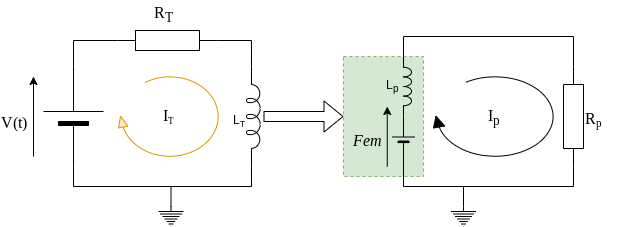
\includegraphics[width=1\textwidth]{Trasformatore/PlasmaCircuit-EquivalentCalc.png}
	\caption[Circuito Equivalente Bobina/Plasma all'interno di un Tokamak trascurando l'induzione del plasma verso la bobina]{Circuito Equivalente Bobina/Plasma semplificato}
\end{figure}


\subsection{Dal circuito alla dinamica}

\subsection{Funzione di Trasferimento}

\newpage


\section{Trasduttore di Corrente}\label{CurrentSense}
Come detto nell'introduzione, l'obiettivo della tesi è di controllare la corrente sul secondario usando il campo elettrico del secondario, la misura della corrente scorrente sul primario in tale ottica non sarebbe una misura di interesse. Essendo però un lavoro di ricerca, si è preferito poter misurare la corrente effettivamente circolante nel Primario del trasformatore, così da poter meglio interpretare i dati di misura senza ambiguità.\\
\begin{figure}[h]
	\centering
	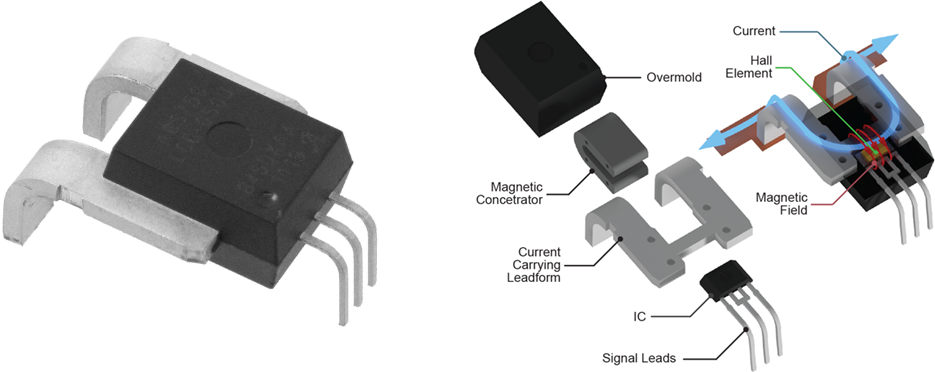
\includegraphics[width=1\textwidth]{ACS770/ACS770-Fig.png}
	\caption[Sensore di Corrente \citefield{ACS770}{series}]{Sensore di Corrente}
\end{figure}
%\vspace{-1cm}
\subsection{Sensore scelto}
Per misurare la corrente del primario, si è posizionato in serie allo stesso il sensore di Corrente \cite{ACS770}.\\
La famiglia di sensori ha in generale le seguenti caratteristiche: \vspace{-5mm}
\begin{center}
	\begin{tabular}[t]{|l r|}
		\hline
		Bandwidth:                             & 120 kHz                               \\
		Output rise time :                     & 4.1 $ \mu s $                         \\
		Ultralow power loss:                   & 100 $ \mu \Omega $ Resistenza Interna \\
		Single supply operation                & 4.5 to 5.5 V                          \\
		Extremely stable output offset voltage &                                       \\
		\hline
	\end{tabular}
\end{center}

\noindent
In oltre, delle tante varianti presenti, si è scelto di usare la \citefield{ACS770}{series}, le cui caratteristiche chiave sono:

\begin{center}
	\begin{tabular}[t]{|l r|}
		\hline
		Primary Sampled Current: & $\pm$ 100 A     \\
		Sensitivity Sens (Typ.)  & 20(mV/A)        \\
		Current Directionality   & Bidirectional   \\
		$T_{OP}$                 & –40 to 150 (°C) \\
		\hline
	\end{tabular}
\end{center}

\noindent
L'ampio margine di misura, e la robustezza alle variazioni di temperatura rendono rendono il dispositivo perfetto per misurare i nostri esperimenti.\\
L'ampio margine di misura permette di comprendere tutti i possibili valori di corrente ottenibili in laboratorio, rendendo il prototipo adatto a scopi futuri.\\
\vspace{-8mm}

\subsection{Criticità}
Unico punto dolente è il suo principio di funzionamento: essendo il sensore basato su un l'effetto Hall, ovvero una misura diretta del campo magnetico indotto dalla corrente nel conduttore, è importante tenere distante il sensore dal Trasformatore Centrale che nei suoi momenti di massimo flusso di corrente, genera ovviamente un campo magnetico non indifferente.

\subsection{Funzionamento Interno}
\vspace{-5mm}
\begin{figure}[h]
	\centering
	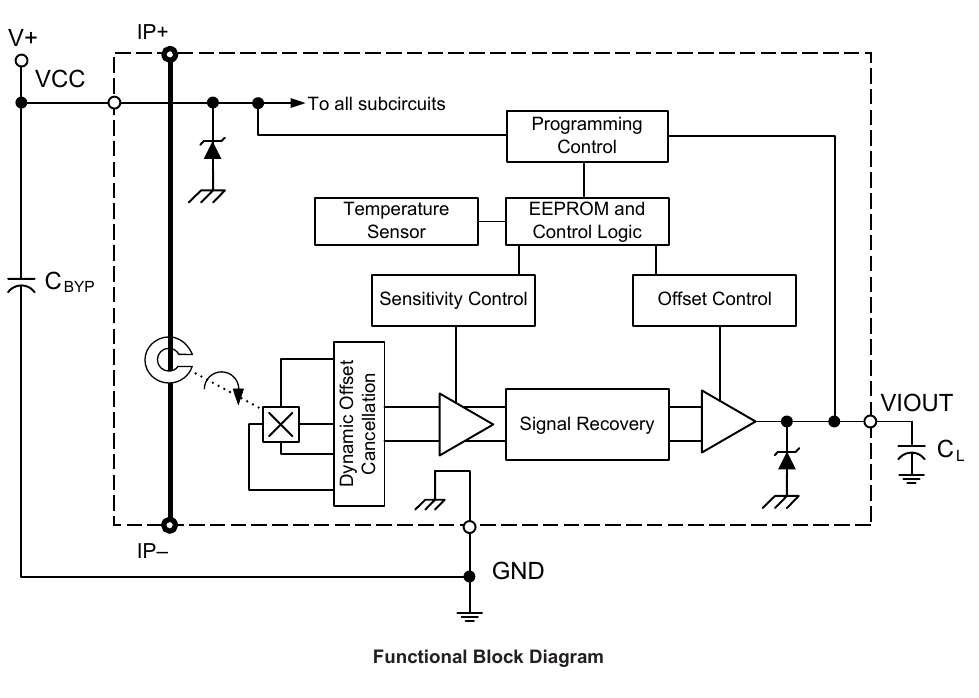
\includegraphics[width=0.8\textwidth]{ACS770/ACS770-SchemaBlocchi.png}
	\caption[\citefield{ACS770}{series} Schema a Blocchi]{Schema a Blocchi}
\end{figure}
\noindent
Tra le caratteristiche chiave dell'\cite{ACS770}, troviamo il disaccoppiamento fisico tra la corrente da misurare e il circuito di misura.\\
Questa caratteristica chiave, garantisce la salvaguardia del circuito logico a valle, dai possibili eventi catastrofici a monte.\\
Esso è in oltre fornito di sensori di temperatura e sistemi di \textit{Signal Recovery} che permettono all'Hardware stesso di compensare parzialmente \nonLinearita termiche e nella misura dell'effetto Hall, ottenendo un output assimilabile a un segnale lineare:

\begin{figure}[h]
	\centering
	\includegraphics[width=1\textwidth]{ACS770/ACS770-Sensibilità.png}
	\caption[\citefield{ACS770}{series} Sensibilità rispetto Temperatura]{Sensibilità}
\end{figure}

\noindent
Come si può vedere dal grafico, gli errori sono tanto più marcati quanto maggiore è la corrente da misurare, ma leggendo dal datasheet abbiamo che questo errore, che dipende si fortemente dalle temperature di esercizio dell'esperimento, non è mai, neanche negli esperimenti più sfortunati, superiore al $\pm2\%$.\\
Anzi, alle temperature $\approx$ 25°, si mantiene contenuto tra $\pm0.5\%$.

\begin{figure}[h]
	\centering
	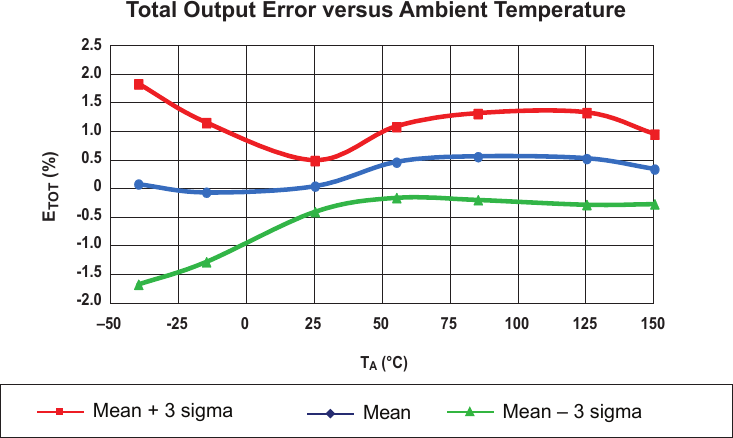
\includegraphics[width=1\textwidth]{ACS770/ACS770-NonLin.png}
	\caption[\citefield{ACS770}{series} \nonLinearita]{Temperatura/NonLinearità}
\end{figure}

\newpage

\subsection{Connessione elettrica}

La connessione del sensore è particolarmente semplice, richiedendo esternamente solo un alimentazione stabilizzata e portando subito in uscita la misura.
\begin{figure}[h]
	\centering
	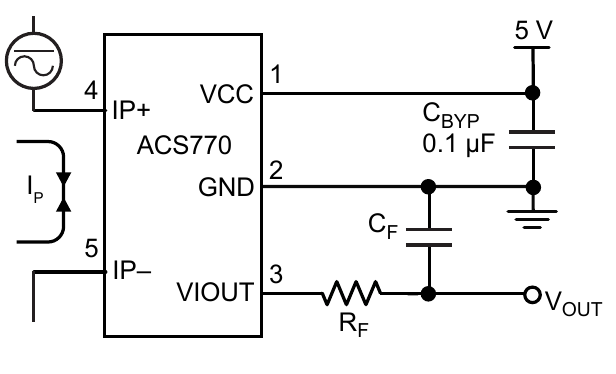
\includegraphics[width=1\textwidth]{ACS770/ACS770-Schema.png}
	\caption[\citefield{ACS770}{series} Schema di collegamento dal Datasheet]{Collegamento dal Datasheet}
\end{figure}

\noindent
Rispetto allo schema proposto dal datasheet, però, si è anche deciso di omettere il filtro passa-basso sulla \textbf{VIOUT}, questa scelta è stata presa per minimizzare il più possibile ritardi di misura della corrente istantanea, poiché le dinamiche del sistema sul secondario, come visto, sono di tipo derivativo, e quindi estremamente rapide.\\

\subsection{Misura}
Il transduttore, misura della corrente sotto forma di tensione, la quale varia in base alla \textbf{Sensibilità} del modello in uso. 
Avendo noi il \citefield{ACS770}{series}, il datasheet riporta:
\begin{center}
	\begin{tabular}[t]{|l r|}
		\hline
		Primary Sampled Current: & $\pm$ 100 A   \\
		Sensitivity Sens (Typ.)  & 20(mV/A)      \\
		Current Directionality   & Bidirectional \\
		\hline
	\end{tabular}
\end{center}

\noindent
Ciò implica che la corrente misurata, è calcolabile come:\\
{\large \begin{center}
	$I_{read} = \frac{V_{Read}[V]}{V_{sense}[V/A]}$
\end{center}
}

\paragraph{Rimozione Offset}
Essendo però il device ad alimentazione singola (0--5V), ma la corrente misurabile Bi-direzionale, sorge la necessità di spostare gli 0A a una tensione superiore agli 0V.\\
Il datasheet riporta che $V_{offset} = \frac{Vcc}{2}\approx$ 2.5V. Da cui deriva che la vera misura di corrente è:
{\LARGE
\begin{empheq}[box=\mathCalc]{equation*}
	I_{read} = \frac{V_{Read}-V_{offset}}{V_{sense}} \frac{V}{[V/A]}
\end{empheq}
}

Al fine di poter misurare l'offset effettivo, durante il set-up viene eseguito a esperimento fermo una misura dell'offset attuale, usando la \nameref{lst:offsetCalc}.\\
Il risultato della computazione, oltre ad essere usato nel controllo è inviato al computer per la post elaborazione dei dati nei grafici.

\paragraph{Analisi Sensibilità}
Usando nell'esperimento un ADC a 10Bit con tensione di riferimento a 5V, abbiamo che la massima sensibilità del \microC, ovvero il suo bit meno significativo è pari a:
%\vspace{-5mm}
\begin{empheq}[box=\mathResult]{equation*}
V_{step}=\frac{Vcc}{2^{10}-1} = 4,887mV
\end{empheq}
\noindent
Il che equivale a una \textbf{Sensibilità di Corrente} del $\mu$Controllore pari a:
%\vspace{-5mm}
\begin{empheq}[box=\mathResult]{equation*}
	I_{step} =\frac{ V_{step}}{V_{sense}} = 244,379 mA
\end{empheq}
\noindent
Il ché rende la misura buona per osservare cosa stia accadendo, ma sicuramente non sufficientemente densa da poterla usare come parametro ingresso di controllo.

\newpage

\section{Driver di Corrente - IBT-2}\label{CurrentDriver}
Per l'attuazione del controllo di corrente nella bobina primaria del trasformatore, è stato usato il driver di corrente \cite{IBT-2} .


\begin{figure}[h]
	\centering
	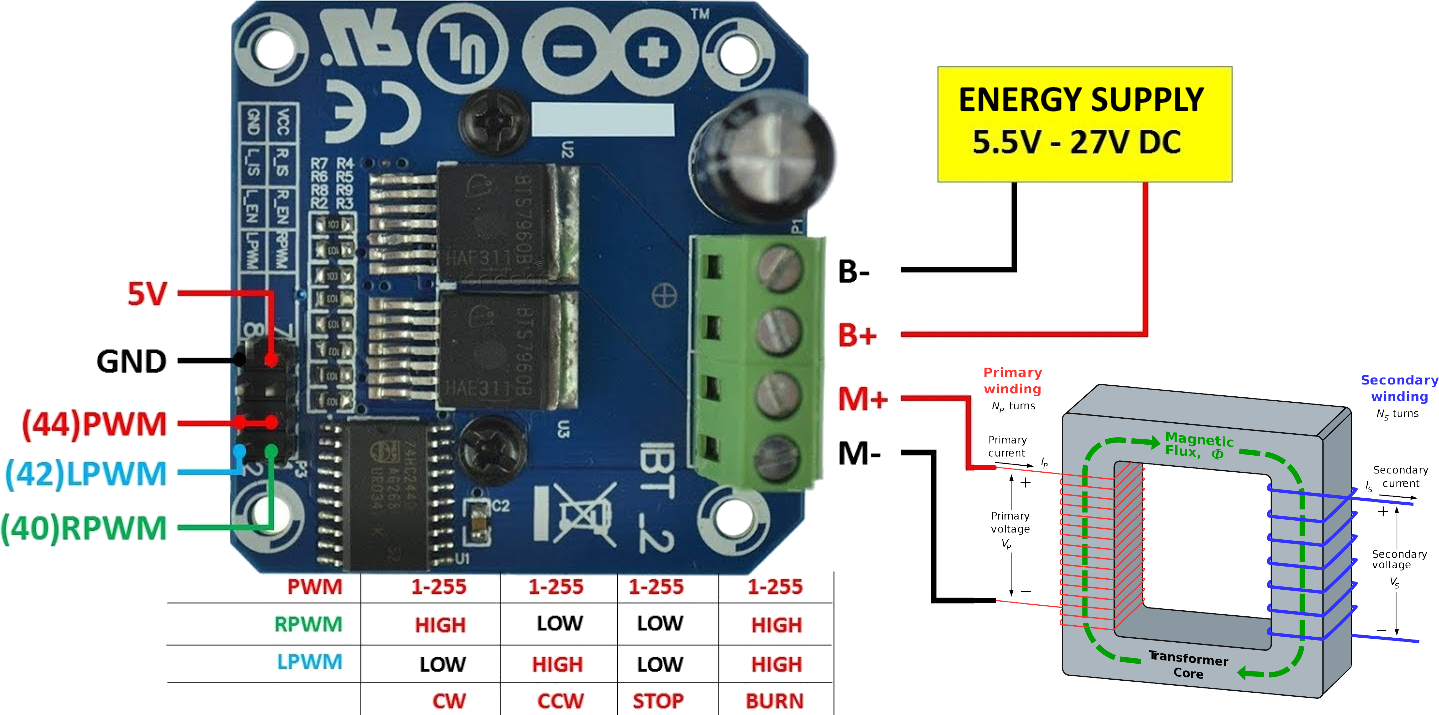
\includegraphics[width=1\textwidth]{IBT-2/TopView.png}
	\caption[Driver Motori IBT-2 TopView \& PinOut]{IBT-2 TopView.}
\end{figure}

\noindent
Esso non è un comune Ponte-H integrato: per poter gestire potenze superiori è stato costruito usando 2 Half-Bridge (\cite{BTS7960b}) collegati assieme mediante una opportuna logica per ricreare un normale Ponte-H.\\
Questa scheda in particola ha prestazioni interessanti per gli scopi di questa tesi, i principali sono elencati di seguito:\vspace{-8mm}
\begin{center}
	\begin{tabular}[t]{|l r|}
		\hline
		Power Input Voltage:                                     & 6 -- 27 V \\
		Peak current:                                            & 43 A      \\
		Massima Frequenza di PWM:                                & 25 kHz    \\
		Protezione Sovra Tensioni                                &           \\
		Disaccoppiamento Ingresso di Potenza/Logica di controllo &           \\
		\hline
	\end{tabular}
\end{center}
\noindent
Di particolare interesse per l'esperimento è proprio la corrente di picco gestibile:
avendo le dinamiche del sistema tempi inferiori ai 5 secondi, poter reggere correnti di picco così elevate rende
la scheda perfetta per i nostri scopi.

\newpage
\subsection{Schema Elettrico}
Al suo interno il driver è composto da 2 Half-Bridge \cite{BTS7960b}, connesse secondo lo schema:
\begin{figure}[h]
	\centering
	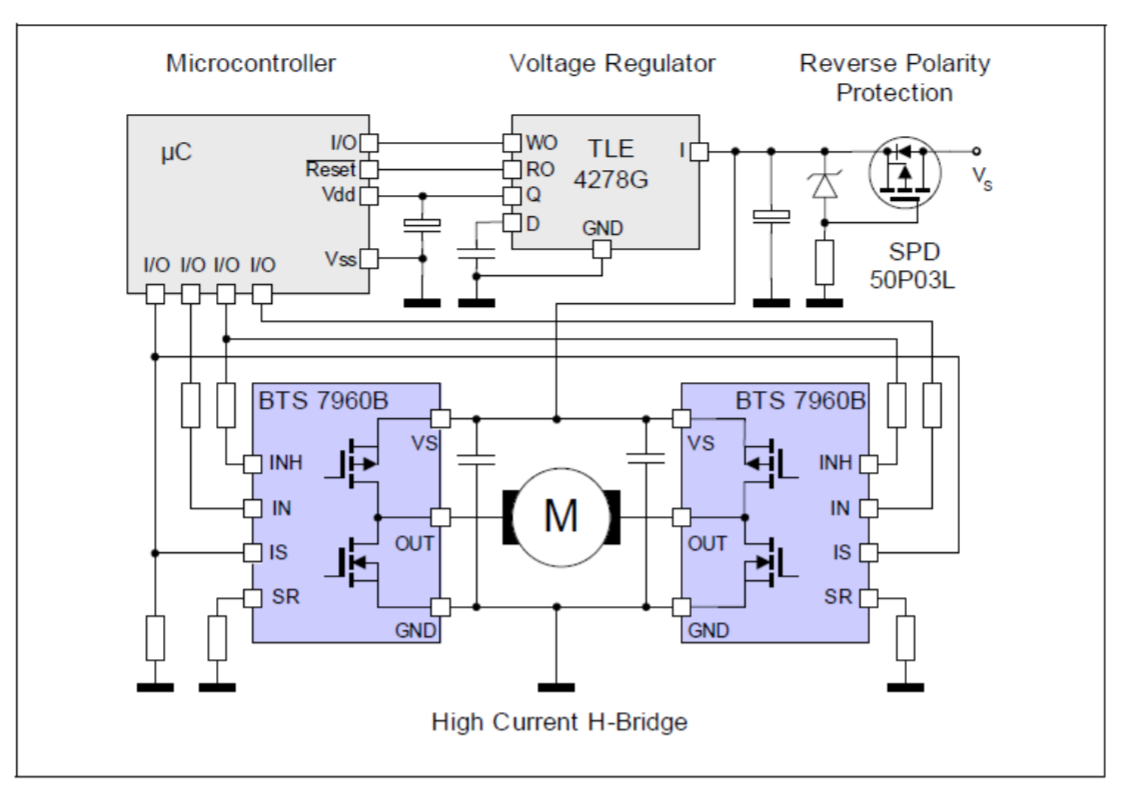
\includegraphics[height=0.5\textheight]{IBT-2/elettricScheme.png}
	\caption[IBT-2 Schema Elettrico]{IBT-2 Schema Elettrico}
\end{figure}\vspace{-5mm}

\noindent
Il \microC è protetto dal carico connesso all'interno del \citefield{BTS7960b}{series}, lasciando al \microC solo il compito di controllare i segnali.


\subsection{Connessione di Controllo}
Il driver permette 2 modalità di funzionamento:
\begin{description}
	\item[Doppio PWM] Modalità operativa che richiede l'uso di 2 PWM\\
	      Ciascun PWM controlla uno dei 2 Half-Bridge, e per evitare di bruciare i driver devono essere controllati singolarmente, il vantaggio di questa configurazione è la possibilità di usare 2 frequenze di controllo diverse.
	\item[Singolo PWM] Modalità operativa classica di un normale Ponte-H\\
	      In questa modalità, la porta nand presente sulla scheda attua la logica di controllo opportuna per governare i 2 Half-Brige come fossero un normale Ponte-H.
\end{description}

\noindent
Per il nostro esperimento si è scelto di usare il collegamento \textbf{\underline{Singolo PWM}} così da evitare spiacevoli sorprese e avere il PWM di controllo sempre sincronizzato.	

\newpage
\subsection{Benchmark Driver}
Il driver sulla carta à buone prestazioni, ma non sono descritte le sue \nonLinearita, per farle risaltare si sono effettuati 2 esperimenti usando differenti input di controllo:
\begin{enumerate}
	\item \nameref{lst:ondaTriangloare} \\ \vspace{-11mm}
	      \begin{figure}[h]
% TODO: Creare grafico 17 senza Errore e Zoomando meglio la deadzone
		      \centering
		      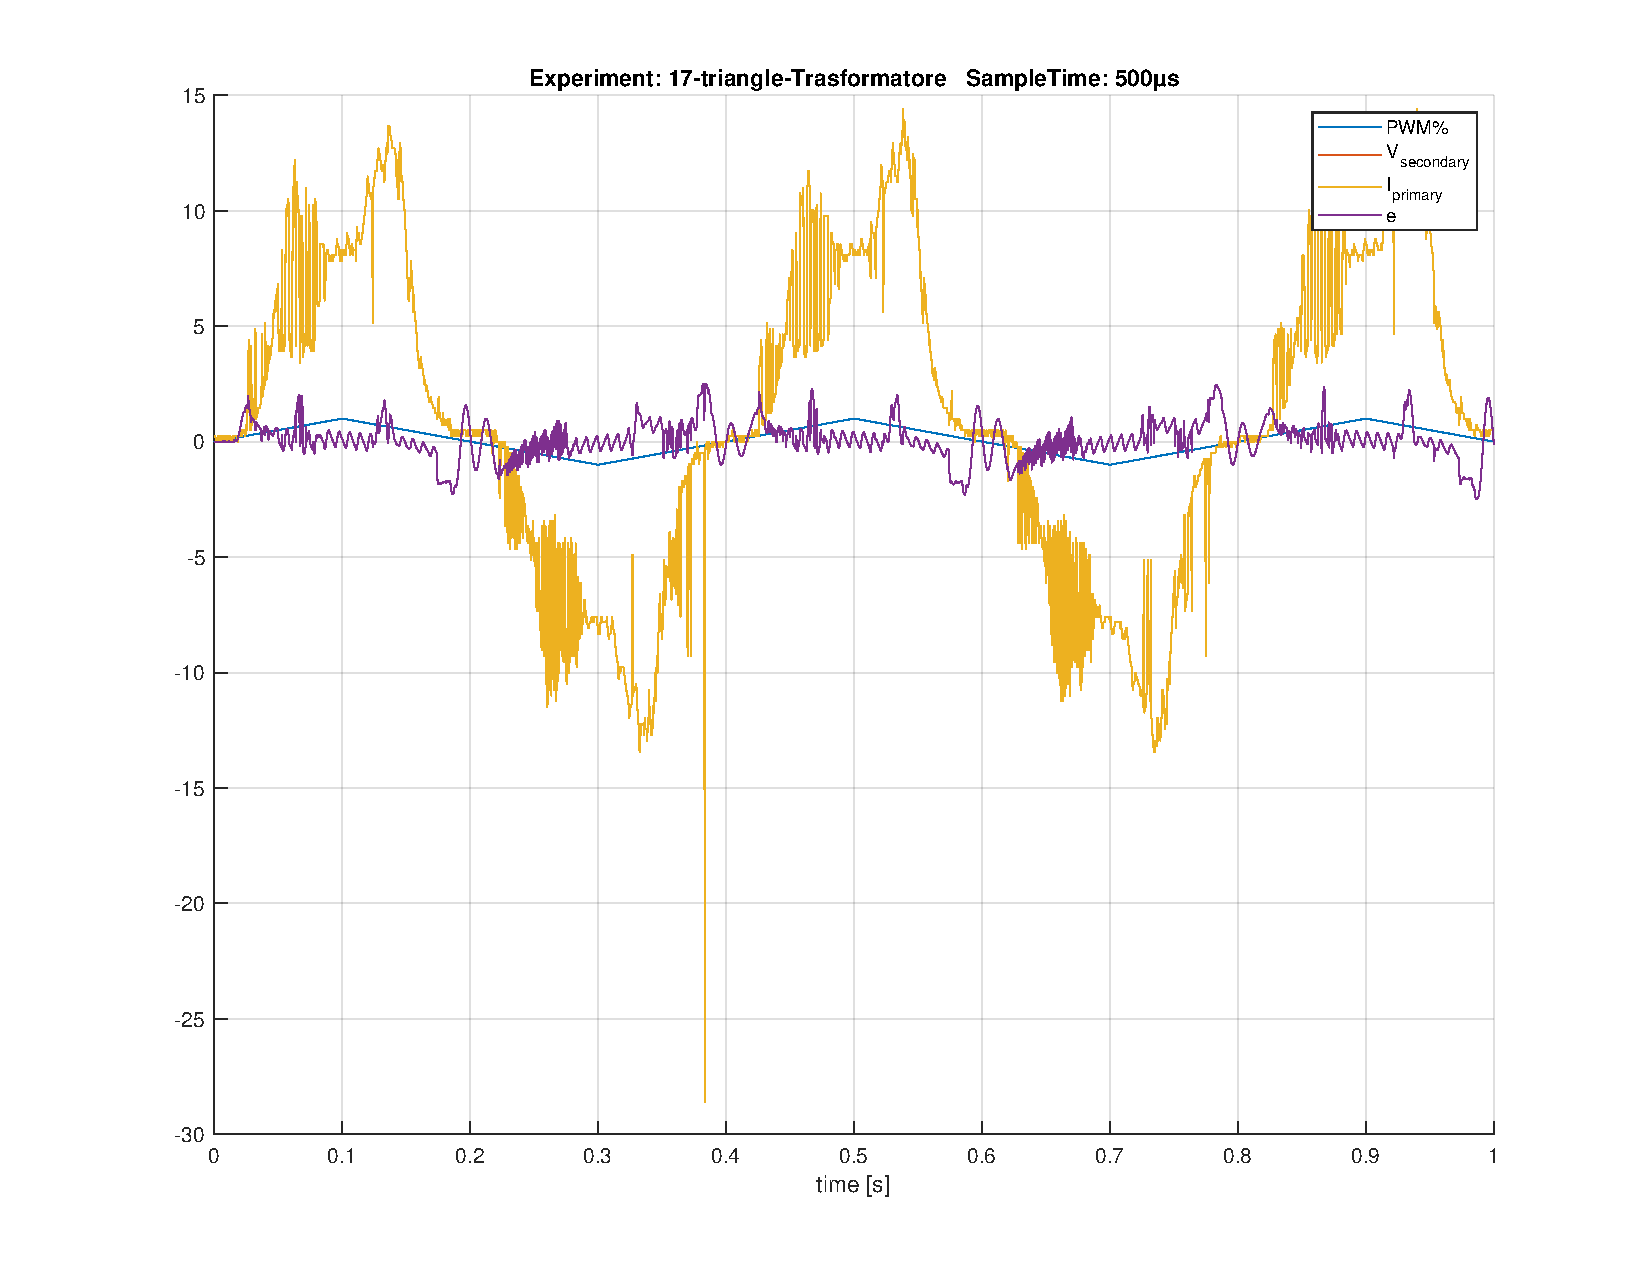
\includegraphics[height=0.5\textheight]{IBT-2/17-triangle-Trasformatore.pdf}
		      \caption[Esperimento con Onda Triangolare]{Onda Triangolare}
	      \end{figure}\vspace{-10mm}
	      \paragraph{Dead-Zone Inferiore} L'onda triangolare si presta bene per far risaltare la problematica della Dead-Zone Inferiore, infatti in tutti gli intorni in cui il segnale passa per 0, è possibile vedere come la corrente non vari minimamente, è però possibile notare che i 2 lati non sono simmetrici tra di loro, questo è facilmente spiegabile dal fatto che il primo ha una condizione iniziale $ \neq $ 0 e di fatto stiamo ancora osservando l'esaurimento del transitorio, la soglia di Dead-Zone Inferiore è quindi calcolata vedendo il primo valore di PWM  per cui il sistema risponde a destra degli 0.      
	      
	      \newpage
	\item \nameref{lst:ondaTrapezoidale} \\
	      \begin{figure}[h]
		      \centering
% TODO: Creare grafico 12 senza Errore e Zoomando meglio la deadzone
		      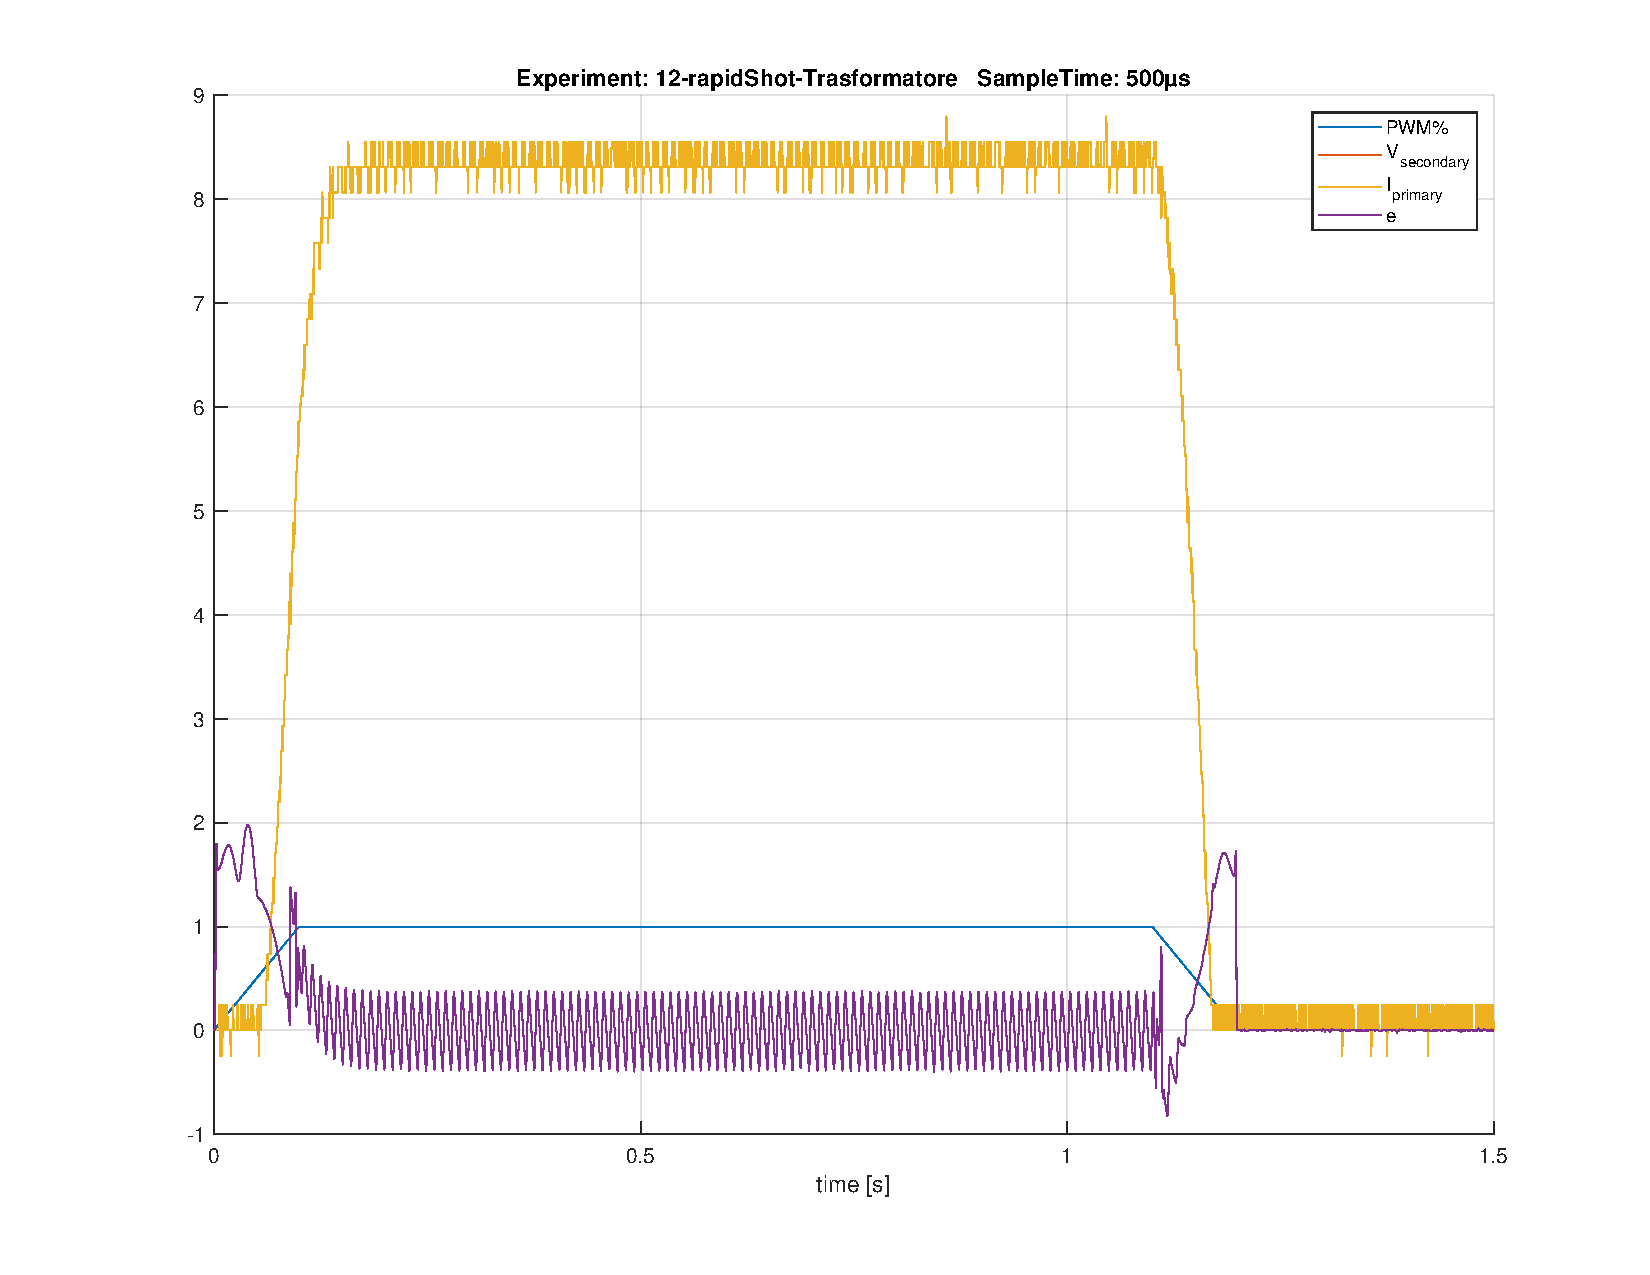
\includegraphics[height=0.5\textheight]{IBT-2/12-rapidShot-Trasformatore.pdf}
		      \caption[Esperimento con Onda Trapezoidale]{Onda Trapezoidale}
	      \end{figure}  \vspace{-10mm}
	      \paragraph{Dead-Zone Superiore} Con questo secondo segnale, si vuole mettere in evidenza il ritardo durante la discesa della rampa, pari a circa 20ms {\small \textit{(guarda 1.1s)}}, questo ritardo è in realtà dovuto da una seconda Dead-Zone presente però ai Duty-Cycle alti del PWM.
	      \vspace{-5mm}
	      \paragraph{Disturbo 50Hz} Essendo in oltre presente un segnale costante per un pò, quando i transitori terminano risulta evidente la presenza della 50hz nel segnale della corrente proveniente dall'alimentatore, questo disturbo è però dovuto alla fonte della corrente, ovvero la 220Vac del laboratorio, il medesimo esperimento realizzato con una batteria ovviamente non ha simili disturbi, ma in fase di test del driver, si è preferito usare un alimentatore da laboratorio.
\end{enumerate}
